\chapter{Introduction}

Sequential model-based optimization is an accurately named process, because it attempts to optimize functions by developing a sequence of models. The broad idea is this: you want to understand some process's global behavior from a few sample points, and you have a limited ability to collect more data--think of additional samples as available, but expensive. This is often the case with processes that are difficult to observe or simulate.

Given a few sample points, you use the available data to develop a model of the process's behavior.  With this model alone, you could perform simple \emph{model}-based optimization, using it to predict the locations of global optima. In \emph{sequential} model-based optimization, however, we use predictive models in a more clever, bootstrapping way: to predict what further data, if collected, would allow us to improve our model---and thus our predictive ability---the most. In other words, each model is used to generate another, better model. Global optima, or at least very good solutions, are then found by recursively improving the predictive ability of a model.

To make this process more tangible, consider the case of gold-mining, which is a surprisingly deep analogy to the kind of data mining which is explored in this thesis. Imagine that you are a gold-miner, and you own a claim to Valley X. You want to understand where in the valley you could find the most gold, where best to start a mine. Your mining company has drilled five exploratory shafts throughout the valley. You make a map of the valley's gold distribution based on these five samples.

Were you, the gold miner, only interested in model-based optimization, you would use this rudimentary map to predict where the most gold in the valley is, and start your mine there. Say, however, that you have enough resources to drill five more exploratory shafts first. The clever miner then asks themself, ``where should I drill the next exploratory shaft, to best learn about where the gold is most concentrated in the valley?" By leveraging what they have learned from the first five data points, the miner finds the region they would like most to learn about. After drilling the sixth hole in this region, the miner can improve their model of the gold distribution yet again, and ask the same question: ``where should I drill next, to best advance my search for the gold optimum?'' The goal of this thesis is to automate this decision-making process.

\section{Black-Box Functions}
A central notion to this thesis is that of black-box functions and their optimization. Though the black-box function is an intuitive concept for many mathematicians and scientists, I have found in discussing this thesis with others that it is an unfamiliar idea to the layperson, so I will spend a moment making all readers fully comfortable with the notion.

Simply put, a black-box function is a mysterious process that turns inputs into outputs. Though its inner workings are unknown to the user, it does operate by some hidden logic. The task of this thesis is to optimize the behavior of this process without direct access to the hidden logic inside the black box.

Imagine a literal black box, with some sort of terminal or opening for receiving inputs. If things are put in this box, it spits something out. This thought experiment is illustrated in Fig. \ref{fig:black_box}.

\begin{figure}[h]
	\centering
	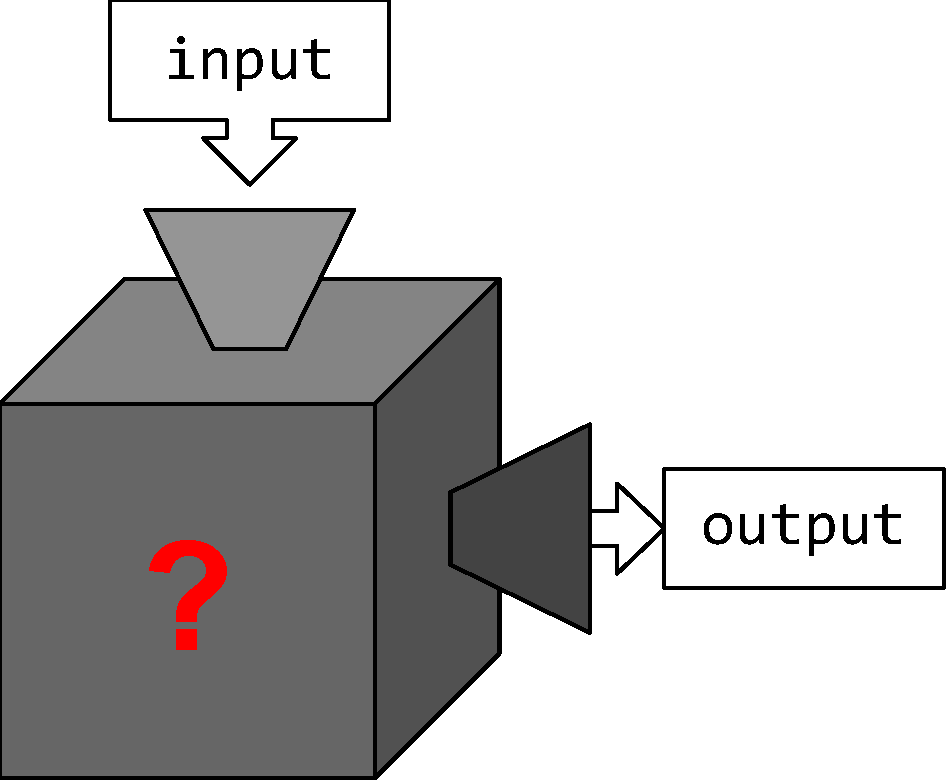
\includegraphics[width=0.5\textwidth]{images/blackbox}
	\caption{A black box: a mysterious but queryable function}
	\label{fig:black_box}

\end{figure}

Now imagine that you are confronted with a black box such as illustrated above, and in particular, one that produces a single numerical output when it is fed input\footnote{In this thesis, we are only concerned with functions that map a $k$-dimensional input to a single-dimensional output, as this is the standard model for optimization.}. Now imagine I were to assign you the task: in only twenty queries of the box, find a particular input that will induce an output greater than 100. How could you go about this task?

To make things easy, we'll make two assumptions about the hidden function in the box: that it is deterministic, so the same input will always produce the same output; and that similar inputs produce similar outputs. This second assumption is crucial, because it allows you to consider observed blackbox values to predict values you have not seen.

Given those two assumptions, no prior knowledge of the blackbox's workings, and the task, ``get the blackbox to produce a desirable output," what does one do? This thesis rigorously addresses that question.

Now this hypothetical, where you have found a magical box that has hidden math inside, and are for some cause compelled to wrench a desirable output from it, sounds somewhat cartoonish and abstract. Yet it is such a general framework that a huge range of real-world problems can be fit into its mould. How often do humans want to control a process that they do not understand, yet can experiment with? Consider the stock market: inputs are your trading decisions, the black box is the market, and the output is your profit. How many people would like a reliable optimization strategy for \emph{that} blackbox function? Many complex biochemical interactions are dynamical enough that they are extremely difficult to model and predict; one iconic example is of protein folding. Here, too, is a setting where inputs (chemical recipes) can be turned into outputs (chemical reagents, or perhaps biomedical results), though the mechanism that accomplishes that transformation (dynamic chemical reaction networks) is somewhat opaque in its inner workings. 

Another major application of blackbox optimizers, which will be explored further in the conclusion, is that of optimizing the parameters of yet other machine learning algorithms. This task, the problem of \emph{hyperparameter optimization}, seeks to optimize the blackbox function which maps algorithm configurations to algorithm performance. Given a machine learning problem, say, identifying dogs in photographs, it is usually fairly straightforward to a practitioner to decide on a class of algorithm that is well-suited to accomplishing that task, e.g., recurrent neural networks. Simply deciding on a class of solution algorithms is not enough to find a solution, however, as there are invariably a basketful of algorithm parameters which must be set before any learning is even to take place. For example, say you want to solve a problem with a so-called deep neural network: how do you decide how many layers of neurons to include? How many neurons should be in each layer? How do you choose an appropriate learning rate? An intuition for questions like these is a large part of what `expertise' means in the field of machine learning, but it is commonly acknowledged that such expertise often errs on artistry rather than science. Because machine learning systems are big, complex, dynamical (and perhaps emergent) systems, is is very hard to know beforehand how well a certain parameter set will solve a given problem or class of problems. Thus, the selection of hyperparameters is another problem space ripe for sequential model-based optimization.

\section{History}

The history of SMBO covers many different applications, with the general trend that the methodology has been developed mainly by engineers, geologists, and practitioners---people who really did have blackbox functions that needed solving---rather than purely theoretical statisticians. The gold-mining example from above was not a didactic invention, no: these methods were really pioneered by miners, geologists, and geostatisticians\footnote{\cite{cressie_kriging_1990}} . Krige himself, a geostatistician, wished to make an `optimal prediction' of the distribution of the `ore grade' of some mineral over a given area, given a relatively small set of sample points\footnote{\cite{krige}}. Though the concept of choosing an optimal next sample was not present from the start, the desire to make rigorously optimal predictions was. This led to the development within kriging of a regression model called the (provably!) ``best linear unbiased predictor'' or BLUP, which in a modern form known as the DACE model is employed by the EGO algorithm, presented in Chapter \ref{ch:ego}.

The EGO algorithm, named for the paper, ``Efficient Global Optimization of Expensive Blackbox Functions,'' \footnote{\cite{jones_efficient_1998}} is a paradigm sequential model-based optimizer\footnote{In the esteem of \cite{hutter_sequential_2011} as well as myself}, though the acronym SMBO did not appear until later. Using a predictive model inherited from the aforementioned geostatistics, the authors of EGO select further samples of the objective function by \emph{maximum expected improvement}, a clever metric which rigorously answers the question, ``where can we sample to learn most about where the global optimum is?'' This topic will discussed rigorously in Section \ref{sec:max_imp}.

 Donald Jones, the lead author of EGO, was working at General Motors R\&D during its writing, and example applications in the paper included the automated design of integrated circuits as well as engine components.

Following the work of Jones and his colleagues, there have been two prominent venues of SMBO-related research. Then first is the company ProtoLife, started by Reed alumni Norman Packard and Mark Bedau, which uses a proprietary SMBO framework called ``Predictive Design Technology'' or PDT to help biochemical and pharmaceutical companies optimize emergent processes such as chemical synthesis \footnote{\cite{protolife_pdt_2013}}. The classic ProtoLife optimization problem goes something like this: Company X has a method for producing a valuable chemical Y. This method is like a recipe: there are a number of different ingredients, to be included in different proportions; instructions for mixing ingredients for a certain amount of time, or heating them to certain temperatures---standard chemistry experiment stuff. We can imagine that if company X were to tweak its recipe, say, heat chemical $a$ to $105^{\circ}$ instead of $100^{\circ}$, or add 5\% more of chemical $b$, they might ultimately produce a larger volume of the valuable product Y. ProtoLife works with customers to parameterize a given chemical recipe along all these dimensions which might be tweaked, and then uses sequential model-based optimization to find the recipe that produces the greatest product with the least amount of effort. This is made possible by laboratory robots that can mechanically make these chemical recipies---embodying a blackbox function that maps recipe descriptions to the actual experimental results of the chemical synthesis so described. 

Another leading figure in modern SMBO research is a person by the name of Frank Hutter, who as far as I can tell, coined the acronym I have so eagerly adopted in his 2009 doctoral dissertation\footnote{\cite{hutter_automated_2009}}. Hutter is interested primarily in SMBO as it pertains to the \emph{algorithm selection problem}, a fascinating application that gets to the core of the field of Machine Learning, and asks, ``given a particular problem, how do you choose which algorithm to use to solve that problem?'' \cite{hutter_sequential_2011} presents an SMBO framework for performing algorithm configuration, with state-of-the-art(-of-the-time) results.




